\textit{Cette partie présente \emph{Hibernate}, l'ORM que nous avons du utiliser pour gérer l'accès aux données. Elle détaille également les différents packages de l'application, la manière dont ont été mappé les informations, la manière adoptée pour la génération du graphe, ainsi que l'utilisation de l'outil développé en ligne de commande.}

\section{L'ORM \emph{Hibernate}}
Hibernate est un framework Java de type ORM. Bien qu'il permette la gestion de la persistance des données (écriture), Hibernate sera utilisé ici uniquement dans le but d'accéder aux métadonnées des SGBD (lecture) via des configurations de Mapping.
\subsection{POJO}
La définition des entités dans \emph{Hibernate} à l'aide de classes \emph{POJO}. Cet acronyme signifiant \og Plain Old Java Object \fg{} fait référence à de simples classes ayant comme principale caractéristique de n'implémenter aucune interface, et de posséder un \emph{getter} et un \emph{setter} par attribut.
\subsection{Mapping}
Le mapping consiste, comme son nom l'indique, à faire la liaison entre les entités définies (classes \emph{POJO}) et les tables en base de données. En règle générale, un objet $x$ est mappé avec une table relationnelle $table-x$, est les attributs $x_1$, $x_2$, \ldots, $x_n$ avec les attributs $tables-x.x_1$, $tables-x.x_1$, \ldots, $tables-x.x_1$. Il est également possible d'ajouter des relations entre attributs (One-to-One, One-to-Many, Many-to-Many), de déclarer des \emph{id}, etc.

\emph{Hibernate} permet de définir le mapping via des annotations directement au sein des classes, ou via des fichiers de configuration xml \texttt{hbm}. C'est cette deuxième méthode que nous avons choisie, et qui sera décrite dans la partie~\ref{section:structure_de_lapplication}.
\subsection{Subselect}

\subparagraph{\ldots}

\section{Structure de l'application}
\label{section:structure_de_lapplication}

\begin{figure}[H]
\centering
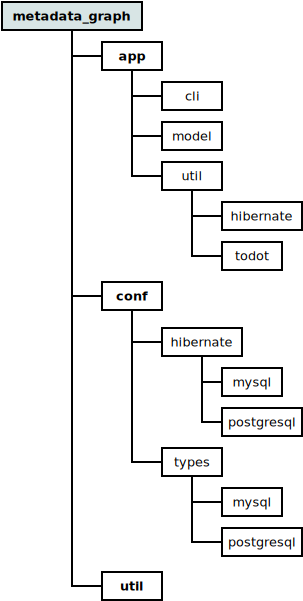
\includegraphics[width=0.5\textwidth]{files/archi}
\caption{Structure des paquets de l'application.}
\label{figure:structure_appli}
\end{figure}

\subsection{Package \emph{Model}}
\subsubsection{Mappings}
\subsubsection{Subselect}
\subsection{Package \emph{toDot}}
\subsubsection{Utilisation de \emph{graphviz}}
dot, neato, etc.
\subsubsection{Génération d'un image du graphe}
\subsection{Package \emph{CLI}}
\subsubsection{Utilisation}
\subsection{Fichiers de configuration}